\begin{figure}[!ht]
\begin{center}
\tikzstyle{stable}=[very thick,blue,samples=201]
\tikzstyle{instable}=[very thick,red,samples=201]
\tikzsetnextfilename{stable-chap0_ext}
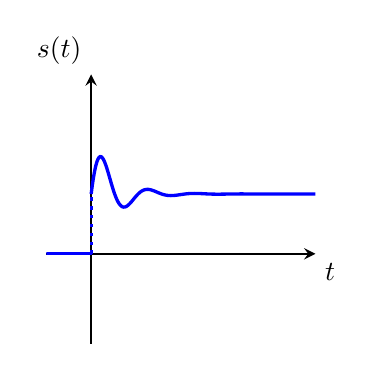
\begin{tikzpicture}
    \begin{axis}
    [   ticks=none,
        axis line style = thick,
        height=5cm,
        width=5cm,
        axis x line=center,
        axis y line=center,
        xmin=-2,
        xmax=10,
        ymin=-1.5,
        ymax=3.0,
        xlabel={$t$},
        ylabel={$s(t)$},
        xlabel style={below right},
        ylabel style={above left},
    ]
    \addplot[stable,domain=-2:0]  {0};
    \addplot[stable,domain=0:10]  {sin(3*deg(x))*exp(-x)+1};
    \draw[dotted,very thick,blue] (axis cs:0,0) -- (axis cs:0,1);
    \end{axis}
\end{tikzpicture}
\tikzsetnextfilename{stable2-chap0_ext}
\begin{tikzpicture}
    \begin{axis}
    [	ticks=none,
        axis line style = thick,
        height=5cm,
        width=5cm,
        axis x line=center,
        axis y line=center,
        xmin=-2,
        xmax=10,
        ymin=-1.5,
        ymax=3.0,
        xlabel={$t$},
        ylabel={$s(t)$},
        xlabel style={below right},
        ylabel style={above left},
    ]
    \addplot[instable,domain=-2:0]  {0};
    \addplot[instable,domain=0:10]  {0.5*x};
    \end{axis}
\end{tikzpicture}

\tikzsetnextfilename{instable-chap0_ext}
\begin{tikzpicture}
    \begin{axis}
    [   ticks=none,
        axis line style = thick,
        height=5cm,
        width=5cm,
        axis x line=center,
        axis y line=center,
        xmin=-2,
        xmax=10,
        ymin=-1.5,
        ymax=3.0,
        xlabel={$t$},
        ylabel={$s(t)$},
        xlabel style={below right},
        ylabel style={above left},
    ]
    \addplot[stable,domain=-2:0] {0};
    \addplot[stable,domain=0:10] {0.5*x};
    \draw[dotted,very thick,blue] (axis cs:0,0) -- (axis cs:0,1);
    \end{axis}
\end{tikzpicture}
\tikzsetnextfilename{instable2-chap0_ext}
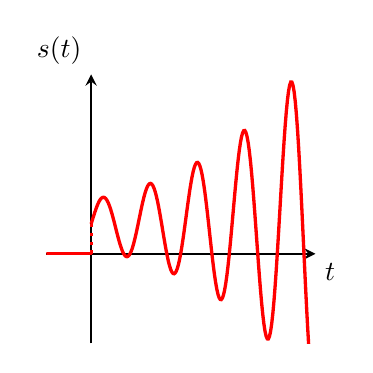
\begin{tikzpicture}%
	\begin{axis}
	[	ticks=none,
        axis line style = thick,
        height=5cm,
        width=5cm,
        axis x line=center,
        axis y line=center,
        xmin=-2,
        xmax=10,
        ymin=-3,
        ymax=6,
        xlabel={$t$},
        ylabel={$s(t)$},
        xlabel style={below right},
        ylabel style={above left},
	]
	\addplot[instable,domain=-2:0] {0};
	\addplot[instable,domain=0:10] {0.8*sin(3*deg(x))*exp(0.2*x)+1};
	\draw[dotted,very thick,red] (axis cs:0,0) -- (axis cs:0,1);
	\end{axis}
\end{tikzpicture}
\caption{Trois exemples de réponses d'un slci à une sollicitation bornée : 
         (en bleu)  réponses stables 
	 (en rouge) réponses instables}
\end{center}                
\end{figure}
